% npuloop 장문판 (학위논문 형식). 4쪽 투고본은 npuloop_esl.tex / npuloop_ko.tex이고 이 파일은 별개다.
%
% 이것은 학위 제출물이 아니다. 그래서 학교·학과·심사위원 인준 페이지가 없다. 표지에는 제목과 저자와
% 날짜만 둔다.
%
%   python paper/make_tables.py --lang ko   # -> tab{1,2,3,4}_rows_ko.tex   (4쪽 원고와 공용)
%   python paper/make_figs.py   --lang ko   # -> fig{1,2}*_ko.pdf           (4쪽 원고와 공용)
%   python paper/make_thesis.py             # -> th_*.tex, fig3_operators_ko.pdf
%   cd paper && lualatex npuloop_thesis && lualatex npuloop_thesis && lualatex npuloop_thesis
%
% 엔진은 lualatex(luatexko). 상호참조와 목차 때문에 세 번 돌린다.
\documentclass[11pt,a4paper,oneside]{report}

\usepackage[margin=30mm,top=32mm,bottom=32mm]{geometry}
\usepackage{luatexko}
\setmainhangulfont{NanumMyeongjo}[ItalicFont=NanumGothic, BoldItalicFont=NanumGothicBold,
                                  SmallCapsFont=NanumMyeongjo]
\setsanshangulfont{NanumGothic}
\setmonohangulfont{NanumGothicCoding}[Scale=MatchLowercase]
\setmainfont{TeX Gyre Termes}
\setsansfont{TeX Gyre Heros}
\setmonofont{TeX Gyre Cursor}[Scale=MatchLowercase]
% 영문 참고문헌의 마침표·쉼표가 CJK 모양이 되지 않도록 끈다.
\hangulpunctuations=0
\hyphenation{gemmlowp}

\usepackage{graphicx}
\usepackage{amsmath}
\usepackage{booktabs}
\usepackage[export]{adjustbox}
% 폭이 본문을 넘는 표만 줄인다. 넘지 않으면 손대지 않으므로 글자 크기가 표마다 튀지 않는다.
\newcommand{\fittable}[1]{\adjustbox{max width=\textwidth}{#1}}
\usepackage{url}
\usepackage{titlesec}
\usepackage[hidelinks]{hyperref}

\renewcommand{\contentsname}{차 례}
\renewcommand{\listfigurename}{그림 차례}
\renewcommand{\listtablename}{표 차례}
\renewcommand{\bibname}{참고문헌}
\renewcommand{\appendixname}{부록}
\renewcommand{\figurename}{그림}
\renewcommand{\tablename}{표}
\renewcommand{\abstractname}{초 록}
% "Chapter 1" 대신 "제 1 장".
\titleformat{\chapter}[display]
  {\normalfont\huge\bfseries}{제 \thechapter 장}{16pt}{\Huge}
\titleformat{name=\chapter,numberless}[display]
  {\normalfont\huge\bfseries}{}{0pt}{\Huge}
\titlespacing*{\chapter}{0pt}{20pt}{28pt}
\renewcommand{\thefigure}{\thechapter.\arabic{figure}}
\renewcommand{\thetable}{\thechapter.\arabic{table}}
\linespread{1.18}

\begin{document}

% ---------------------------------------------------------------- 표지
\begin{titlepage}
\centering
\vspace*{50mm}
{\LARGE\bfseries 모의 양자화와 정수 실행의 격차를\\[4pt] 연산자 단위로 측정하기\par}
\vspace{10mm}
{\large Measuring the Fake-Quantization-to-Integer Gap,\\[2pt] Operator by Operator\par}
\vspace{6mm}
{\large INT8 NPU 배포를 위한 비트 정확 정수 엔진과 그 위에서의 측정\par}
\vfill
{\large \textsc{[저자 성명]}\par}
\vspace{4mm}
{\large 2026년 9월\par}
\vspace{10mm}
{\small 저장소 \url{https://github.com/sokldjs554/npuloop}\par}
\vspace{20mm}
\end{titlepage}

\pagenumbering{roman}
\setcounter{page}{1}

% ---------------------------------------------------------------- 초록
\chapter*{초 록}
\addcontentsline{toc}{chapter}{초록}

INT8 가속기에 신경망을 올리는 작업은 서로 다른 두 프로그램을 다룬다. 판단에 쓰이는 쪽은 양자화--역양자화
노드를 삽입한 부동소수점 그래프, 곧 모의(fake) 양자화이고, 장치에서 실제로 도는 쪽은 int8 가중치와 int32
누산기와 고정소수점 곱셈-시프트 재양자화로 이루어진 정수 프로그램이다. 현업은 둘을 바꿔 써도 되는 것으로
다루지만, 그 가정이 어디까지 성립하는지는 정확도 이외의 축에서 측정된 바가 없다.

이 논문은 그 격차를 연산자 단위로 측정한다. 먼저 TensorFlow Lite 참조 커널과 비트 단위로 일치하는 정수
엔진을 만들고, TensorFlow Lite 완전 정수 모델의 스케일과 영점으로 정수 그래프를 세워 $1000$장의 모든
텐서에서 일치함을 확인해 측정 기준을 외부에 고정했다. 그 위에서 모의 양자화 그래프와 정수 실행의 차이를
연산자 자신의 정수 연산이 만드는 몫(국소 불일치, 교사 강제로 분리)과 종단간 실행에서 살아남는 몫(전파
불일치)으로 나누어, 신경망 7종과 양자화 방식 2종에 대해 전체 테스트셋에서 대응 표준오차와 함께 보고한다.

결과는 세 가지다. 첫째, 정확도는 맞고 텐서는 틀린다. 모의 대 정수 top-1 차이는 모두 $0.20$~\%p 이내이고
12개 $95\%$ 신뢰구간이 전부 0을 포함하는 반면, 출력 코드는 $28.5$--$72.7\%$가 다르고 이미지의
$95$--$100\%$에서 코드가 최소 하나 다르다. 둘째, 격차를 옮기는 연산자는 하나가 아니다. LayerNorm을 빼면
모든 연산자의 국소 불일치가 자기 코드의 $1\%$ 미만이고 그 어긋남은 예외 없이 최하위 비트 $\pm 1$이다.
가장 큰 국소 원천인 정수 LayerNorm($24.77\%$)을 정수에 충실한 모듈로 교체해 $0.00\%$로 만들어도 전파된
출력 불일치는 $72.7\%$에서 $65.7\%$로만 내려간다. 셋째, 이 분리는 분류 과제의 인공물이 아니다. argmax가
없는 초해상 신경망에서도 품질 지표(PSNR)는 $6\times10^{-4}$~dB 안쪽으로 충실한 반면 내보내는 픽셀 코드의
$6.3$--$18.2\%$가 다르다.

아울러 정확도 대리지표가 값을 매기지 못하는 구현 선택을 정량화한다. 재양자화의 반올림을 산술 시프트로
바꾸면 18개 (모델, 시드, 방식) 조합 전부에서 $0.90$--$3.37$~\%p를 잃으며, 그 손해의 부호는 시드를 넘어
옮겨 가지만 크기는 옮겨 가지 않는다. 마지막으로, 밀집 출력 과제를 추가하는 과정에서 측정 도구 자체의
정밀도 결함 하나가 드러났고 그 진단과 수정을 함께 기록한다. 본문의 모든 수치는 공개된 결과 파일에서
스크립트가 생성하며, 지속적 통합이 커밋마다 그 일치를 강제한다.

\bigskip
\noindent\textbf{주제어}: 양자화, 정수 연산, 임베디드 추론, 신경망 처리 장치, 재현성

% ---------------------------------------------------------------- 차례
\tableofcontents
\listoffigures
\listoftables

\clearpage
\pagenumbering{arabic}
\setcounter{page}{1}

% ================================================================ 1
\chapter{서론}

INT8 가속기에 신경망을 올리는 일은 서로 다른 두 프로그램이 결정한다. 질문에 답하는 쪽은 양자화--역양자화
(``모의 양자화'') 노드가 삽입된 부동소수점 그래프이고, 그 정확도가 곧 양자화 정확도로
보고된다~\cite{jacob2018,krishnamoorthi2018}. 실제로 출하되는 쪽은 정수 프로그램이다. int8 가중치, int32
누산기, 고정소수점 곱셈-시프트 재양자화로 이루어진다~\cite{gemmlowp}. 현업은 둘을 바꿔 써도 되는 것으로
다루고, 정확도에 관한 한 대체로 그렇다~\cite{nagel2021}.

그러나 시뮬레이터에 요구되는 것이 정확도뿐인 것은 아니다. 실리콘 브링업과 컴파일러 검증에는 \emph{골든
벡터}, 곧 장치가 내놓아야 할 정수 텐서 그 자체가 필요하다. 학습 후 양자화에서 회귀가 생겼을 때 추적하려면
\emph{어느} 연산자에서 격차가 시작되었는지를 알아야 한다. 둘 다 텐서에 관한 질문이고, 저자가 아는 한 어느
쪽도 측정된 바 없다. 공개된 양자화 벤치마크는 격차를 정확도로 환산해 보고하며~\cite{mqbench}, 배포
툴체인의 계층별 오차 분석은 양자화된 계층이 \emph{부동소수점} 대응물에서 얼마나 떨어져 있는지를 잰다.
시뮬레이터가 \emph{정수 실행}에서 얼마나 떨어져 있는지는 그 사이에서 빠져 있다.

이 논문의 기여는 넷이다. 첫째, 모의 양자화와 정수 실행의 차이를 연산자 단위로 분해하는 측정 방법을
제시한다. 교사 강제로 분리한 \emph{국소} 불일치는 연산자 자신의 정수 연산이 만드는 몫을, \emph{전파}
불일치는 종단간 실행에서 살아남는 몫을 나타낸다. 둘째, 그 분해를 신경망 7종과 양자화 방식 2종에 걸쳐 전체
테스트셋에서 수행하고, 정확도 일치와 텐서 일치가 두 자릿수 이상 분리되어 있음을 대응 표준오차와 함께
보인다. 셋째, 가장 자연스러운 수리 방법 --- 가장 큰 국소 원천 하나에서 시뮬레이터가 장치의 정수 연산을
쓰게 하는 것 --- 을 직접 시험하여, 국소 격차는 완전히 닫히지만 전파 격차는 거의 닫히지 않음을 보인다.
넷째, 정확도 대리지표가 볼 수 없는 재양자화 구현 선택을 시드를 바꿔 가며 정량화한다.

측정이 성립하려면 기준이 되는 정수 엔진 자체가 의심스럽지 않아야 한다. 이 논문의 엔진은 서로 독립인 두
구현(NumPy와 C++)이 모든 중간 텐서에서 일치할 것을 테스트가 강제하고, 파이썬을 쓰지 않는 세 번째 실행기가
직렬화된 파일로부터 같은 코드를 재현하며, 무엇보다 자기 자신이 아니라 TensorFlow Lite 참조 커널이라는 외부
오라클에 대해 검증된다(5.7절). 5장의 모든 수치는 이 엔진 위에서 나온 것이다.

\medskip
이 논문의 구성은 다음과 같다. 2장은 INT8 정수 데이터패스와 모의 양자화의 관계, 그리고 관련 연구를
정리한다. 3장은 연산자별 불일치를 먼저 분류해 문제의 모양을 드러낸다. 4장은 측정 방법을, 5장은 실험
결과를, 6장은 타당성 위협과 측정이 찾아낸 구현 결함을 다루고, 7장에서 정리한다.

% ================================================================ 2
\chapter{배경}

\section{INT8 정수 데이터패스}

정수 추론의 한 계층은 세 단계로 이루어진다. int8 입력 코드와 int8 가중치를 곱해 int32 누산기에 모으고,
int32 바이어스를 더하고, 결과를 다음 계층의 int8 격자로 되돌리는 재양자화를 거친다. 재양자화는 실수 배율을
Q31 고정소수점 승수 $q$와 시프트 $n$으로 근사한다.
\[
  M = \frac{s_{\text{in}}\, s_w}{s_{\text{out}}}
    \;\approx\; q \cdot 2^{-31} \cdot 2^{-n}.
\]
계산은 gemmlowp/TensorFlow Lite의 \texttt{MultiplyByQuantized\-Multiplier}~\cite{gemmlowp}를 따른다. 이
함수는 포화 반올림 배증 상위곱과 2의 거듭제곱 반올림 나눗셈의 합성이며, 둘 다 정확히 정의된 정수 연산이다
(부록~\ref{app:datapath}). 곧 ``INT8''이라는 말이 가리키는 산술은 유일하지 않고, 승수 폭·누산기 폭·반올림
방식이 모두 구현이 고르는 값이다.

활성함수는 데이터패스에 따라 두 갈래로 갈린다. ReLU 계열은 재양자화의 clamp 경계에 흡수되므로 별도의
연산이 필요 없고, SiLU나 GELU처럼 단조롭지만 닫힌 형태가 없는 함수는 256개 항목의 int8 룩업 테이블로
구현한다. 후자는 입력 쪽에 양자화기가 하나 더 붙는다는 뜻이고, 이 차이는 그래프의 양자화 지점 배치를
바꾼다. 평균 풀링은 입력 스케일을 그대로 유지한 채 정수 누적과 나눗셈으로 처리한다.

\section{모의 양자화와 정수 실행}

모의 양자화 그래프는 텐서를 양자화 격자에 맞춰 반올림하고 자른 뒤 다시 부동소수점으로 돌아온다. 곧
$\hat{x} = s\,(\mathrm{clip}(\mathrm{round}(x/s) + z,\ q_{\min},\ q_{\max}) - z)$이고, 이후의 모든 연산은
여전히 float32로 돈다. 정수 프로그램은 대신 int8 코드를 끝까지 유지하고 위의 곱셈-시프트로 다시
스케일한다. 두 프로그램은 \emph{의도}에서는 일치한다. 같은 스케일, 같은 영점, 같은 가중치를 쓴다. 그러나
연산의 순서와 정밀도가 다르므로 최하위 비트마다 어긋날 자유를 갖는다.

이 자유가 실제로 얼마나 쓰이는지가 이 논문의 주제다. 구체적으로 두 가지를 구별해야 한다. 한 연산자의
정수 커널이 \emph{같은 입력}을 받고도 시뮬레이터와 다른 출력을 내는 몫과, 앞에서 생긴 차이가 뒤로
전달되며 커지는 몫이다. 4.3절은 이 둘을 각각 국소 불일치와 전파 불일치로 정의한다.

\section{관련 연구}

MQBench~\cite{mqbench}는 학술 양자화와 배포 가능한 백엔드 사이의 격차를 측정하되 그것을 정확도로
보고한다. 양자화 백서들~\cite{nagel2021,krishnamoorthi2018}은 모의 양자화를 정수 파이프라인의
시뮬레이션으로 다루며, 그 시뮬레이션이 얼마나 충실한지는 다루지 않는다. 배포 툴체인의 계층별 오차 분석은
양자화된 계층이 부동소수점 대응물에서 얼마나 떨어져 있는지를 신호 대 잡음비로 잰다. 이 논문의 측정은
종류가 다르다. 시뮬레이터가 장치에서 실제로 일어나는 정수 실행에서 얼마나 떨어져 있는지를, 신호 대
잡음비가 아니라 코드 단위로 잰다.

정수만 쓰는 트랜스포머 추론은 정수 LayerNorm과 소프트맥스 커널을 이미 확립했다~\cite{ibert,fqvit}. 그
연산자에 대한 이 논문의 기여는 커널이 아니라, 커널과 시뮬레이터가 어긋나는 크기이고 그것을 고치는 것만으로는
충분하지 않다는 증거다(5.3절). 누산기 폭은 학습 시 제약으로 연구되어 왔다~\cite{a2q}. 여기서 재는 축은 그
대신 재양자화 단계의 반올림, 즉 순수한 구현 선택이다(5.5절). 비용 모델 쪽에서는 SCALE-Sim~\cite{scalesim}과
같은 사이클 정확 시뮬레이터가 표준이며, 5.7절에서 이 논문의 분석 모델을 그 도구 및 Arm Vela에 대조한다.

% ================================================================ 3
\chapter{동기: 격차는 어디에 있는가}

모의 양자화가 정수 실행을 얼마나 못 맞히는지를 묻기 전에, 못 맞히는 곳이 어디인지를 먼저 보아야 한다.
``INT8 실행이 부정확하다''는 말은 설계 지침이 되지 못한다. 어떤 연산자가 얼마나 어긋나는지를 알아야
무엇을 고칠지, 고쳐서 될 일인지를 판단할 수 있다.

\section{연산자별 불일치 분류}

표~\ref{tab:operators}와 그림~\ref{fig:operators}는 이 논문이 다루는 신경망 7종 전부에 대해, 각 노드의
정수 커널에 시뮬레이터의 입력 코드를 먹이고(교사 강제) 그 노드의 출력만 비교한 결과를 연산자 종류별로
모은 것이다. 측정 절차는 4.3절에 있다. 여기서는 분포만 본다.

\begin{table}[!t]
\caption[연산자별 국소 불일치]{연산자별 국소(교사 강제) 불일치. 신경망 7종 × 양자화 방식 2종의 모든 노드를 연산자 종류로 모은
것이다. ``불일치 노드''는 국소 불일치가 0보다 큰 노드의 수, ``국소 최대 $|\Delta|$''는 그 노드들에서
관측된 코드 차이의 최댓값(LSB), ``전파 최대''는 같은 노드에서 종단간 실행이 만든 불일치의 최댓값이다.}
\label{tab:operators}
\centering
\small
\fittable{\setlength{\tabcolsep}{5pt}
\begin{tabular}{lrrrcrr}
\toprule
연산자 & 노드 & 불일치 노드 & 국소 평균(\%) & 국소 범위(\%) & 국소 최대 $|\Delta|$ & 전파 최대(\%) \\
\midrule
LayerNorm & 26 & 26 & 24.766 & 23.637--26.226 & 1 & 82.8 \\
평균 풀링 & 12 & 12 & 0.989 & 0.100--2.697 & 1 & 55.9 \\
소프트맥스 & 12 & 12 & 0.500 & 0.276--0.798 & 1 & 26.7 \\
행렬곱 & 24 & 24 & 0.273 & 0.076--0.425 & 1 & 75.6 \\
합성곱 & 286 & 286 & 0.163 & 0.020--0.928 & 1 & 73.2 \\
선형 & 84 & 84 & 0.139 & 0.031--0.960 & 1 & 80.8 \\
잔차 덧셈 & 106 & 5 & $<$0.001 & 0.000--0.001 & 1 & 75.6 \\
LUT 활성함수 & 50 & 0 & 0 & 0 & 0 & 39.5 \\
연결(concat) & 6 & 0 & 0 & 0 & 0 & 11.3 \\
\bottomrule
\end{tabular}
}
\end{table}

\begin{figure}[!t]
\centering
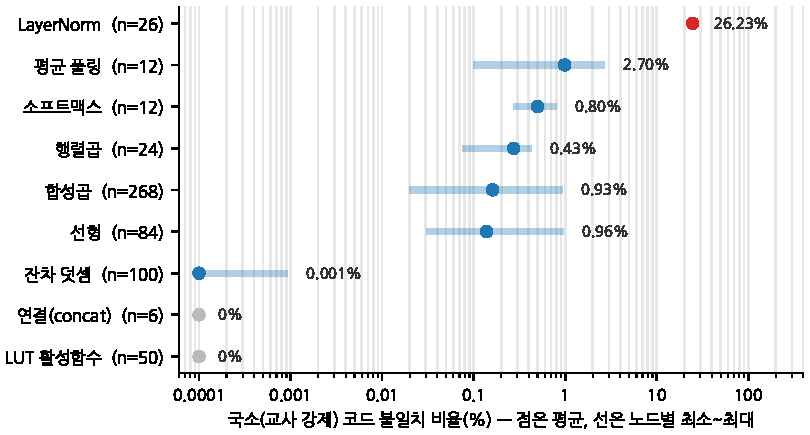
\includegraphics[width=\textwidth]{fig3_operators_ko.pdf}
\caption[연산자별 국소 불일치 분포]{연산자별 국소 불일치 분포. 가로축은 로그 눈금이며, 국소 불일치가 정확히 0인 연산자(LUT
활성함수, 연결)는 축 왼쪽 끝에 회색으로 붙여 표시했다.}
\label{fig:operators}
\end{figure}

분포는 두 무리로 갈린다. 정수 LayerNorm은 자기 코드의 평균 $24.77\%$에서 어긋나고, 나머지 모든 연산자는
$1\%$ 미만이다. 그 사이에 두 자릿수의 간격이 있고, 중간에 놓인 연산자는 없다. 평균 풀링이 $0.99\%$로
두 번째지만 이는 반올림 동점 때문이며, 합성곱 $0.16\%$, 선형 $0.14\%$, 행렬곱 $0.27\%$, 소프트맥스
$0.50\%$가 그 아래에 모여 있다.

크기보다 중요한 것은 \emph{어긋남의 종류}가 하나뿐이라는 사실이다. 표~\ref{tab:operators}의 ``국소 최대
$|\Delta|$'' 열은 예외 없이 $1$이다. LayerNorm까지 포함해, 교사 강제로 잰 모든 불일치는 최하위 비트
$\pm 1$이다. 정수 커널이 크게 틀리는 경우는 관측되지 않았고, 다만 $\pm 1$이 얼마나 자주 일어나는지가
연산자마다 다를 뿐이다.

세 종류의 연산자는 정확히 $0\%$다. int8 룩업 테이블 활성함수 50개 전부, 연결(concat) 6개 전부, 그리고
reshape·transpose 같은 구조 연산이다. 룩업 테이블은 입력 코드에서 출력 코드로 가는 결정적 사상이므로
시뮬레이터와 엔진이 같은 표를 쓰는 한 어긋날 수 없고, 연결과 구조 연산은 코드를 옮길 뿐 산술을 하지
않는다. 잔차 덧셈 $100$개 중 $95$개도 $0$이고, 나머지 $5$개는 원소 $100$만 개당 몇 개 수준
($0.00005$--$0.00093\%$)에서만 어긋난다.

\section{무엇이 문제인가}

이 분류가 곧바로 말해 주는 것이 둘 있다.

첫째, \textbf{고칠 대상이 뚜렷하다}. 트랜스포머를 INT8로 옮기는 실무자에게 ``LayerNorm을 가장 먼저
의심하라''는 지침은 이 표에서 바로 나온다. 다른 연산자보다 두 자릿수 큰 국소 원천이 하나뿐이기 때문이다.

둘째, \textbf{고쳐도 될지는 이 표만으로 알 수 없다}. 국소 불일치는 각 연산자를 고립시켜 잰 값이고,
같은 표의 ``전파 최대'' 열은 전혀 다른 그림을 보여 준다. 국소 불일치가 정확히 $0$인 LUT 활성함수의 전파
불일치가 $39.5\%$까지 올라가고, 잔차 덧셈은 $75.6\%$까지 간다. 자기는 아무것도 틀리지 않았는데 앞에서 온
$\pm 1$을 그대로 실어 나른 것이다. 그러므로 가장 큰 국소 원천을 없애면 전파 격차가 그만큼 줄어드는지는
따로 시험해야 한다. 5.3절이 그 시험이다.

% ================================================================ 4
\chapter{방법}

\section{그래프 IR과 정수 그래프 export}

\texttt{torch.fx}로 추적한 그래프에서 BatchNorm을 합성곱에 접고 shape를 전파해 정적 그래프를 만든다.
지원 연산자는 합성곱(깊이별 포함), 선형, 덧셈, 곱셈, 연결, 행렬곱, 소프트맥스, LayerNorm, 풀링,
활성함수, transpose, reshape, flatten이고, 그 밖의 노드를 만나면 조용히 근사하지 않고 즉시 실패시킨다.
측정 도구에서는 침묵하는 폴백이 가장 위험한 동작이기 때문이다.

캘리브레이션을 마친 모의 양자화 그래프는 정수 그래프로 export된다. 가중치는 int8, 바이어스는 int32, 그리고
출력 채널별 Q31 승수와 시프트가 붙는다. ReLU 계열 활성함수는 이 단계에서 재양자화의 clamp로 흡수되고,
LUT 활성함수는 256항목 표로 구워진다.

\section{정수 엔진과 외부 검증}

실행은 2.1절의 gemmlowp/TensorFlow Lite 의미론을 따른다. 엔진은 세 겹으로 검증된다.

\textbf{내부 일치.} 서로 독립으로 작성한 NumPy 구현과 C++ 구현이 \emph{모든} 중간 텐서에서 일치할 것을
테스트 스위트가 강제한다. 어느 한쪽의 실수는 다른 쪽과의 불일치로 드러난다.

\textbf{직렬화 왕복.} 정수 그래프를 파일로 내보내고, 파이썬을 쓰지 않는 독립 C++ 실행기가 그 파일만으로
같은 코드를 재현한다. 파이썬 런타임에 숨은 상태가 없음을 보인다.

\textbf{외부 오라클.} 가장 중요한 겹이다. TensorFlow Lite의 완전 정수 모델을 가져와 \emph{그}
스케일·영점·가중치·바이어스로 정수 그래프를 세우고, TensorFlow Lite 참조 커널과 출력을 비교한다. 결과는
5.7절에 있다. 자기 자신에 대한 일치는 구현이 일관되다는 것만 보이지만, 외부 런타임과의 비트 일치는 이
논문이 ``정수 실행''이라 부르는 것이 실제 배포 런타임이 하는 일과 같음을 보인다.

\section{국소 불일치와 전파 불일치}

한 장의 이미지에 대해, 모의 양자화 그래프가 노드 $n$에서 만드는 코드를 $f_n$(양자화기 출력을 정수 코드로
환산한 것), 정수 엔진을 종단간으로 돌렸을 때 같은 노드에서 나오는 코드를 $i_n$이라 하자. 노드 $n$의
\emph{전파} 불일치는 $f_n \neq i_n$인 원소의 비율이다.

\emph{국소} 불일치는 노드 $n$의 정수 커널에 입력으로 $f$의 코드, 곧 \emph{시뮬레이터가 그 자리에서 내놓은
코드}를 먹이고(교사 강제) 그 노드의 출력만 비교한 것이다. 상류에서 온 오차가 제거되므로, 남는 차이는 그
연산자 자신의 정수 산술이 만든 것이다.

두 값은 서로를 보완한다. 국소 불일치만 보면 어떤 커널이 문제인지 알 수 있지만 그것이 결과에 얼마나
기여하는지는 알 수 없고, 전파 불일치만 보면 결과는 알 수 있지만 원인을 지목할 수 없다. 3장의 표에서 두 열이
전혀 다른 순위를 보인 것이 그 때문이다.

\section{LayerNorm 정수 에뮬레이션}

3장의 분류는 LayerNorm을 지목한다. 진단이 맞는지 확인하는 가장 직접적인 방법은 원인을 없애 보는 것이다.
\texttt{emulate\_integer\_layernorm}은 캘리브레이션된 모의 양자화 그래프의 \texttt{nn.LayerNorm}을, 입력
코드 위에서 정수 엔진과 \emph{같은 함수}(int64 합, 정확한 정수 제곱근, Q15 정규화, 채널별 Q31 재양자화)를
수행하는 모듈로 바꾼다. 구성상 비트 단위까지 같고, 내보내는 정수 프로그램은 바뀌지 않는다. 실험은 후자를
단언(assert)한다. 곧 두 조건 사이에서 달라지는 것은 시뮬레이터뿐이다.

\section{통계 처리}

정확도 차이는 대응 표본으로 다룬다. 같은 이미지를 세 번(부동소수점, 모의 양자화, 정수) 평가하고, 이미지별
정답 여부 차이의 평균을 표준오차 $s/\sqrt{n}$ 및 $95\%$ Wald 구간과 함께 보고한다. 두 독립 표본의 차이로
다루면 표준오차가 과대평가되므로, 같은 이미지에서 잰 차이를 쓰는 것이 중요하다.

초해상처럼 이미지당 연속값(PSNR)으로 채점하는 과제에는 같은 방식의 연속형 대응 차이를 쓴다. 이미지별
차이의 평균과 그 표준오차, $95\%$ 구간을 보고한다.

% ================================================================ 5
\chapter{성능 평가}

\section{실험 설정}

CIFAR-10 신경망 5종을 학습해 기준선으로 삼는다(표~\ref{tab:baselines}). ReLU를 쓰는 ResNet-20과 SiLU를 쓰는
ResNet-20, MobileNetV2-0.5(깊이별 합성곱), 분기를 연결하는 Inception 계열 CNN, 그리고 ViT-128/6(어텐션 블록
12개, LayerNorm 13개)이다. 여기에 Imagenette를 $128\times128$로 쓰는 신경망 2종을 더한다. ResNet-20과,
5.4절의 초해상 신경망이다.

학습 $50{,}000$장은 고정 시드로 학습 $45{,}000$장과 검증 $5{,}000$장(클래스별 $500$장, 층화)으로 한 번
나눈다. 체크포인트 선택은 검증 분할로만 하고 test $10{,}000$장은 선택된 체크포인트에 대해 마지막에 한 번
평가한다. 캘리브레이션 이미지도 학습 분할에서만 뽑는다.

학습 후 양자화 방식은 둘이다. 채널별 가중치에 비대칭 활성화를 쓰는 방식(\textsc{pc})과 텐서별 가중치를
쓰는 방식(\textsc{pt})이며, 둘 다 학습 이미지 $512$장으로 보정했다. 학습과 평가는 모두 CPU 4코어에서
수행했다.

\begin{table}[!t]
\caption[CIFAR-10 기준선]{CIFAR-10 기준선. 사이클과 배열 활용률은 가상 NPU 비용 모델(\texttt{tiny-1tops} 스펙)의 값이므로
측정값이 아니라 추정값이다. lint 점수는 NPU 준비도 정적 분석의 종합 점수다.}
\label{tab:baselines}
\centering
\small
\fittable{\setlength{\tabcolsep}{5pt}
\begin{tabular}{lrrrrrr}
\toprule
모델 & 파라미터 & MACs & float32 top-1(\%) & 사이클 & 배열 활용률(\%) & lint 점수 \\
\midrule
ResNet-20 ReLU & 272,474 & 40.8M & 89.59 & 87.7k & 45.4 & 92.9 \\
ResNet-20 SiLU & 272,474 & 40.8M & 90.34 & 90.7k & 44.0 & 75.3 \\
MobileNetV2-0.5 & 700,490 & 28.0M & 90.23 & 200.5k & 12.1 & 88.2 \\
ViT-128/6 & 810,890 & 57.0M & 80.98 & 164.6k & 33.8 & 75.3 \\
Inception-32 & 423,066 & 54.0M & 89.59 & 99.1k & 53.2 & 97.0 \\
\bottomrule
\end{tabular}
}
\end{table}

정확도 열은 따로 적지 않으면 전체 테스트셋 기준이다(CIFAR-10 $10{,}000$장, Imagenette $3{,}925$장).
노드별 분해는 고정된 $250$장 배치를 쓰며, 입력이 $64$픽셀보다 큰 신경망은 $125$장(초해상은 $64$장)을
쓴다.

\section{정확도와 텐서의 분리}

표~\ref{tab:fidelity}이 핵심 측정이다. 모의 대 정수 정확도 차이의 최댓값은 $0.20$~\%p,
$|\Delta|/\mathrm{SE}$의 최댓값은 $1.6$이며, 12개 신뢰구간이 모두 0을 포함한다. 이 표본 크기에서 정확도
대리지표는 정확한 것과 구별되지 않고, 이미지 단위 top-1 일치율은 $97.9$--$99.7\%$다.

\begin{table}[!t]
\caption[모의 양자화 대 정수 실행, 전체 테스트셋]{모의 양자화 대 비트 단위로 일치하는 정수 실행, 전체 테스트셋. \textsc{pc}는 채널별 가중치,
\textsc{pt}는 텐서별 가중치. $\Delta$는 같은 이미지에서 잰 (정수 $-$ 모의) top-1이며 대응 표준오차를 함께
적었다. ``코드''는 서로 다른 출력 로짓 코드의 비율, ``이미지''는 코드가 하나라도 다른 이미지의 비율이다.}
\label{tab:fidelity}
\centering
\footnotesize
\fittable{\input{tab1_rows_ko}}
\end{table}

같은 행이 텐서에서는 어긋난다. 출력 로짓 코드의 $28.5\%$(Inception-32)에서 $72.7\%$(ViT-128/6)가 다르고,
이미지의 $95$--$100\%$에서 코드가 최소 하나 다르다. 트랜스포머가 극단이기는 하나 예외는 아니다. CNN들이
$50$--$63\%$, 입력이 더 큰 Imagenette 모델이 $36\%$에 자리한다.

그림~\ref{fig:decomposition}은 이 결과를 노드 단위로 펼친 것이다. 국소 불일치는 3장에서 본 대로 작고
평평한 반면, 전파 불일치는 첫 합성곱에서부터 --- 12개 행 전부에서 첫 격차가 그 노드다 --- 단조롭게 올라가
출력에서 $28$--$73\%$에 이른다. 정확도가 $99\%$ 일치한다는 보고는 시뮬레이터가 검증 벡터를 공급할 수
있다는 증거가 되지 못한다.

\begin{figure}[!t]
\centering
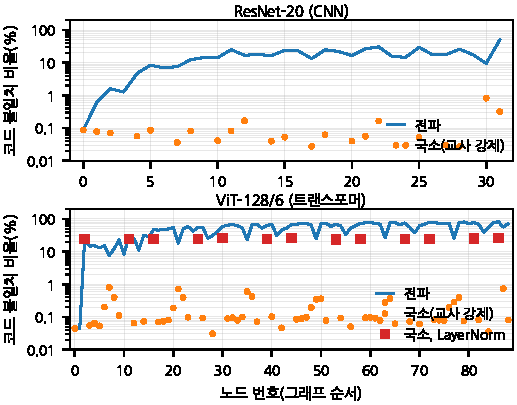
\includegraphics[width=0.92\textwidth]{fig1_decomposition_ko.pdf}
\caption[노드별 코드 불일치]{노드별 코드 불일치, \textsc{pc} 방식. 국소(교사 강제) 불일치는 LayerNorm을 뺀 모든 연산자에서
$1\%$ 미만이고, 전파 불일치는 첫 합성곱에서 시작해 출력의 $50$--$73\%$까지 올라간다. 세로축은 로그
눈금이며, 국소 불일치가 0인 노드는 그리지 않았다.}
\label{fig:decomposition}
\end{figure}

\section{LayerNorm 어블레이션}

격차가 연산자별 오차의 합이라면 가장 큰 항을 없앴을 때 그만큼 줄어야 한다. 4.4절의 에뮬레이션으로 이를
직접 시험한다.

표~\ref{tab:layernorm}이 결과다. LayerNorm의 국소 불일치는 $24.77\%$에서 정확히 $0.00\%$로 내려가고 로짓
절대차 평균은 약 $23\%$ 개선된다. 그러나 전파된 출력 코드 불일치는 $72.7\%$에서 $65.7\%$로만 움직인다
(텐서별은 $72.6\% \rightarrow 66.0\%$). 정확도는 어느 방향으로든 대응 표준오차 두 배 안쪽에서 움직이므로
개선으로 읽을 수 없다.

\begin{table}[!t]
\caption[LayerNorm 정수 에뮬레이션]{시뮬레이터의 LayerNorm을 정수에 충실하게 바꾼 결과(ViT-128/6, $10{,}000$장). 각 방식의 두 행
사이에서 정수 프로그램은 바뀌지 않았고 시뮬레이터의 LayerNorm만 다르다. 로짓 절대차 평균은 \textsc{pc}에서
$0.119 \rightarrow 0.091$, \textsc{pt}에서 $0.118 \rightarrow 0.093$으로 줄어든다.}
\label{tab:layernorm}
\centering
\footnotesize
\fittable{\setlength{\tabcolsep}{4pt}
\begin{tabular}{llcccc}
\toprule
방식 & LayerNorm & 국소(\%) & 코드(\%) & 일치(\%) & $\Delta$ (\%p) \\
\midrule
\textsc{pc} & float32 & 24.77 & 72.7 & 97.93 & $+0.10\pm0.13$ \\
\textsc{pc} & 정수 (13개) & 0.00 & 65.7 & 98.29 & $+0.25\pm0.11$ \\
\textsc{pt} & float32 & 24.76 & 72.6 & 98.07 & $+0.20\pm0.12$ \\
\textsc{pt} & 정수 (13개) & 0.00 & 66.0 & 98.60 & $+0.13\pm0.10$ \\
\bottomrule
\end{tabular}
}
\end{table}

가장 큰 국소 원천 하나를 완전히 없애도 전파 격차의 10분의 1 정도만 회수된다. 남는 것이 개별적으로는 코드의
$1\%$ 미만에서만 어긋나는 연산자들의 $\pm 1$ LSB 사건이 증폭된 결과이기 때문이다. 3.2절에서 유보했던 질문에
대한 답은 ``아니오''다. 비트 정확한 검증 벡터는 정수 구현에서 나와야 하며, 부동소수점 시뮬레이터를 연산자
하나씩 고쳐 나가는 길은 대체재가 되기에 너무 느리게 수렴한다.

\section{출력 텐서가 결과물인 과제}

5.2절과 5.3절의 신경망은 모두 분류기여서 출력 텐서와 답 사이에 argmax가 하나 서 있다. 코드가 수십 퍼센트
달라도 top-1은 거의 움직이지 않으므로, ``텐서는 못 맞힌다''는 결론의 \emph{결과}를 보여줄 수가 없다. 이
절은 argmax를 걷어낸다.

ESPCN~\cite{espcn}은 부분 픽셀 초해상 신경망이다. 합성곱 3개로 Imagenette를 $64 \rightarrow 128$로 올리며,
출력이 곧 그림 그 자체다. 파라미터 $8{,}796$개로 30 epoch(CPU 8.4분) 학습해 test PSNR $30.23$~dB를 얻었고,
최근접 이웃 확대의 $27.26$~dB보다 $2.97$~dB 높다. 새 연산자 지원은 필요 없었다. 픽셀 셔플을
view/permute/reshape로 쓰면 IR이 이미 가진 reshape와 transpose로 내려간다.

\begin{table}[!t]
\caption[밀집 출력 과제: ESPCN $\times 2$]{출력 텐서가 결과물인 과제: Imagenette에서의 ESPCN $\times 2$, 이미지 $3{,}925$장, 이미지당 출력값
$49{,}152$개. PSNR은 $[0,1]$ 범위의 dB이며 배포와 똑같이 출력을 clip한 뒤 이미지별로 재고 평균했다.}
\label{tab:dense}
\centering
\footnotesize
\fittable{\input{tab4_rows_ko}}
\end{table}

표~\ref{tab:dense}는 같은 그림을 반복한다. 양자화 비용은 $0.279$~dB(\textsc{pc})와 $0.667$~dB(\textsc{pt})
이고 시뮬레이터는 그 비용을 $6\times10^{-4}$~dB 안쪽으로 맞힌다. 이 표본 크기에서는 분해되는 차이지만
($|\Delta|/\mathrm{SE} = 17.6$) 맞히려는 비용보다 세 자릿수 작다. 그런데도 출력 픽셀 코드의 $6.3\%$와
$18.2\%$가 $3{,}925$장 전부에서 다르고, 최대 3레벨까지 벌어진다.

연산자별 구조는 CNN과 같다. 합성곱의 국소 불일치는 $0.06$--$0.40\%$이고 모두 최하위 비트 $\pm 1$이며, 첫
분기점도 첫 합성곱이다. 전파 값이 분류기($28$--$73\%$)보다 작은 것은 이 신경망이 3층이라는 깊이 효과이지
과제의 성질이 아니다. 요컨대 정확도 일치와 텐서 일치의 분리는 분류 과제의 인공물이 아니며, 시뮬레이터는
기준 로짓 벡터를 공급할 수 없듯이 기준 이미지도 공급할 수 없다.

\section{재양자화 반올림과 시드}

재양자화의 곱셈-시프트는 반올림 단계로 끝나는데, 구현에 따라 이를 단순 산술 시프트로 바꾸고 싶은 유혹이
있다. 정확도 대리지표는 이 선택에 값을 매기지 못한다. 그림~\ref{fig:rounding}과 표~\ref{tab:rounding}은 그
선택을 기준 구현과 비교해 전체 테스트셋에서, 신경망당 독립적으로 학습한 체크포인트 3개로 측정한 것이다.

\begin{figure}[!t]
\centering
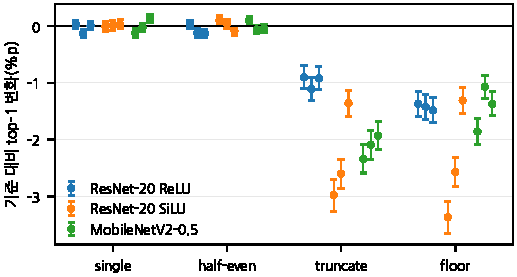
\includegraphics[width=0.92\textwidth]{fig2_rounding_ko.pdf}
\caption[반올림 방식 대비 top-1 변화]{기준 재양자화 반올림 대비 top-1 변화, 전체 테스트셋, 신경망당 독립적으로 학습한 체크포인트
3개(오차 막대는 대응 표준오차).}
\label{fig:rounding}
\end{figure}

\begin{table}[!t]
\caption[반올림 방식의 손해, 시드 3개]{기준 구현 대비 반올림 방식의 손해, 시드 3개의 평균 $\pm$ 표준편차(\%p).}
\label{tab:rounding}
\centering
\footnotesize
\fittable{\setlength{\tabcolsep}{4pt}
\begin{tabular}{lccc}
\toprule
반올림 & ResNet-20 ReLU & ResNet-20 SiLU & MobileNetV2-0.5 \\
\midrule
\texttt{single} & $-0.03\pm0.09$ & $+0.01\pm0.02$ & $-0.00\pm0.13$ \\
\texttt{half\_even} & $-0.07\pm0.09$ & $+0.02\pm0.09$ & $+0.00\pm0.09$ \\
\texttt{truncate} & $-0.98\pm0.12$ & $-2.31\pm0.85$ & $-2.12\pm0.21$ \\
\texttt{floor} & $-1.42\pm0.06$ & $-2.42\pm1.04$ & $-1.43\pm0.40$ \\
\bottomrule
\end{tabular}
}
\end{table}

결과는 둘이다. 첫째, \textbf{부호와 유의성은 시드에 강건하다}. \texttt{truncate}와 \texttt{floor}는 18개
(모델, 시드, 방식) 조합 전부에서 기준보다 나빴고, 그 폭은 $0.90$--$3.37$~\%p,
$|\Delta|/\mathrm{SE}$는 $4.4$에서 $11.8$ 사이였다. 반면 단일 반올림과 짝수 반올림 경로는 잡음 범위를
벗어나지 않는다($|\Delta| \leq 0.13$~\%p). 둘째, \textbf{크기는 옮겨 가지 않는다}. ResNet-20 SiLU에서
\texttt{truncate}의 손해는 시드 3개에 걸쳐 $1.36$에서 $2.98$~\%p까지 벌어져 시드 표준편차가 효과 크기의
$37\%$에 이르는 반면, ResNet-20 ReLU는 효과의 10분의 1 이내에 머문다. 두 편향 방식 중 어느 쪽이 더
나쁜지도 연산의 성질이 아니라 신경망의 성질이다. ResNet-20 ReLU는 세 시드 모두에서 \texttt{floor}가,
MobileNetV2는 세 시드 모두에서 \texttt{truncate}가 더 많이 잃는다. 반올림 방식의 비용을 시드 하나의 수치로
인용해서는 안 된다.

\section{정수 구현 세부의 비용}

반올림은 재양자화가 고르는 여러 값 중 하나일 뿐이다. 표~\ref{tab:requant}는 나머지 세 축 --- 승수 폭,
누산기 폭, 바이어스 폭 --- 을 기준 설정(Q31 승수, int32 누산기, int32 바이어스) 대비로 잰 것이다.

\begin{table}[!t]
\caption[재양자화 구현 세부의 비용]{재양자화 구현 세부의 정확도 비용. 기준 설정 대비 정수 top-1 변화(\%p), 이미지 $2{,}000$장,
\texttt{npu-default} 스킴. 설정 이름의 \texttt{m}은 승수 비트, \texttt{acc}는 누산기 비트, \texttt{b}는
바이어스 비트다.}
\label{tab:requant}
\centering
\small
\fittable{\setlength{\tabcolsep}{4pt}
\begin{tabular}{llccc}
\toprule
축 & 설정 & ResNet-20 ReLU & ResNet-20 SiLU & MobileNetV2-0.5 \\
\midrule
곱셈기 비트 & \texttt{tflite-m31-acc32-b32} & 기준 & 기준 & 기준 \\
 & \texttt{tflite-m15-acc32-b32} & $+0.10$ & $+0.00$ & $-0.25$ \\
 & \texttt{tflite-m7-acc32-b32} & $+0.25$ & $+0.00$ & $+0.00$ \\
 & \texttt{tflite-m3-acc32-b32} & $-8.20$ & $-2.00$ & $-1.55$ \\
누산기 비트 & \texttt{tflite-m31-acc24-b32} & $+0.00$ & $+0.00$ & $+0.00$ \\
 & \texttt{tflite-m31-acc20-b32} & $+0.00$ & $+0.00$ & $+0.00$ \\
 & \texttt{tflite-m31-acc16-b32} & $-73.30$ & $-31.55$ & $-73.80$ \\
바이어스 비트 & \texttt{tflite-m31-acc32-b16} & $-10.55$ & $-0.80$ & $-0.15$ \\
 & \texttt{tflite-m31-acc32-b12} & $-76.65$ & $-71.20$ & $-73.45$ \\
\bottomrule
\end{tabular}
}
\end{table}

승수 폭은 관대하다. Q31에서 Q15로 내려도 정확도가 거의 움직이지 않으며, 무너지는 것은 Q7 이하다. 누산기와
바이어스 폭은 그렇지 않다. 이 축들은 5.5절의 반올림 축과 달리 시드 하나로만 측정했으므로, 부호는 몰라도
크기는 신뢰구간과 함께 읽어야 한다. 6.1절에 이 한계를 적었다.

\section{외부 대조: TensorFlow Lite와 Arm Vela}

\subsection*{TensorFlow Lite 참조 커널}

표~\ref{tab:tflite}는 4.2절의 외부 검증 결과다. TensorFlow Lite 완전 정수 모델의 스케일·영점·가중치·바이어스로
정수 그래프를 세우고 $1{,}000$장을 흘렸을 때, 합성곱과 풀링이 기존 방식의 이중 반올림을 쓰고 완전 연결
계층이 단일 반올림을 쓰는 조합에서 모든 텐서가 완전히 일치한다. NumPy 엔진과 C++ 엔진이 같은 값을 낸다.

\begin{table}[!t]
\caption[TensorFlow Lite 참조 커널 교차 검증]{TensorFlow Lite 참조 커널과의 교차 검증. 이미지 $1{,}000$장, 출력 원소 $10{,}000$개.
\texttt{tflite+fc-single}은 합성곱·풀링이 이중 반올림, 완전 연결 계층이 단일 반올림을 쓰는 조합이다.}
\label{tab:tflite}
\centering
\small
\fittable{\setlength{\tabcolsep}{4pt}
\begin{tabular}{llcccc}
\toprule
반올림 조합 & 엔진 & 불일치 이미지 & 불일치 원소 & top-1 일치(\%) & 완전 일치 \\
\midrule
\texttt{tflite+fc-single} & numpy & 0 / 1000 & 0 / 10000 & 100.0 & 예 \\
\texttt{tflite+fc-single} & cpp & 0 / 1000 & 0 / 10000 & 100.0 & 예 \\
\texttt{tflite} & numpy & 20 / 1000 & 20 / 10000 & 100.0 & 아니오 \\
\texttt{tflite} & cpp & 20 / 1000 & 20 / 10000 & 100.0 & 아니오 \\
\texttt{single} & numpy & 155 / 1000 & 337 / 10000 & 100.0 & 아니오 \\
\texttt{single} & cpp & 155 / 1000 & 337 / 10000 & 100.0 & 아니오 \\
\texttt{half\_even} & numpy & 182 / 1000 & 364 / 10000 & 100.0 & 아니오 \\
\texttt{half\_even} & cpp & 182 / 1000 & 364 / 10000 & 100.0 & 아니오 \\
\texttt{truncate} & numpy & 1000 / 1000 & 8203 / 10000 & 99.8 & 아니오 \\
\texttt{truncate} & cpp & 1000 / 1000 & 8203 / 10000 & 99.8 & 아니오 \\
\texttt{floor} & numpy & 1000 / 1000 & 7968 / 10000 & 99.8 & 아니오 \\
\texttt{floor} & cpp & 1000 / 1000 & 7968 / 10000 & 99.8 & 아니오 \\
\bottomrule
\end{tabular}
}
\end{table}

이 기준이 얼마나 빡빡한지에 대한 눈금이 하나 있다. 같은 모델에서 TensorFlow Lite 자신의 최적화
델리게이트(XNNPACK)와 참조 커널은 $1{,}000$장 중 $155$장, 출력 원소 $10{,}000$개 중 $337$개에서 서로 다른
답을 낸다. 곧 ``TensorFlow Lite와 비트가 맞는다''는 말조차 어느 커널을 가리키는지 밝히지 않으면 성립하지
않는다. 표의 나머지 행은 반올림 방식을 바꿨을 때 일치가 어떻게 깨지는지를 보여 준다. \texttt{truncate}와
\texttt{floor}는 $1{,}000$장 전부에서 어긋난다.

\subsection*{비용 모델}

비용 모델 쪽 대조는 두 가지다. SCALE-Sim v3(사이클 정확, weight-stationary)와는 신경망 4종 × 배열 크기
3종에서 합계 사이클이 $0.08\%$ 이내로 일치한다. Arm Vela(Ethos-U55-256)와는 합성 망 5종에서
표~\ref{tab:vela}와 같이 갈린다.

\begin{table}[!t]
\caption[Arm Vela(Ethos-U55-256) 대조]{Arm Vela(Ethos-U55-256)와의 대조. 같은 INT8 그래프에 대한 두 분석 추정기의 값이며, 비율은
npuloop/Vela다. 둘 다 추정값이고 실측이 아니다.}
\label{tab:vela}
\centering
\small
\fittable{\setlength{\tabcolsep}{5pt}
\begin{tabular}{lrrrrr}
\toprule
합성 망 & Vela MACs & npuloop MACs & Vela 사이클 & npuloop 사이클 & 비율 \\
\midrule
\texttt{conv-stack} & 3.06M & 3.06M & 47.8k & 40.2k & 0.840 \\
\texttt{dw-separable} & 0.43M & 0.43M & 22.4k & 10.7k & 0.477 \\
\texttt{pointwise-heavy} & 1.81M & 1.79M & 44.4k & 12.7k & 0.286 \\
\texttt{wide-late} & 2.77M & 2.77M & 61.5k & 50.6k & 0.822 \\
\texttt{deep-narrow} & 0.79M & 0.79M & 15.8k & 11.3k & 0.711 \\
\bottomrule
\end{tabular}
}
\end{table}

MAC 수는 사실상 같지만 사이클은 $0.29$--$0.84$배로, npuloop 쪽이 일관되게 낙관적이다. 격차가 가장 큰
\texttt{pointwise-heavy}는 $1\times1$ 합성곱이 대부분인 망이고, 가장 작은 \texttt{conv-stack}은 일반
합성곱이 대부분이다. 곧 이 비용 모델은 배열 채움·비움과 가중치 교체 비용을 과소평가하며, 그 과소평가가
계층 모양에 따라 달라진다. 6.1절에 한계로 적었고, 본문에서 사이클을 인용할 때는 언제나
\texttt{simulated} 라벨을 붙인다.

% ================================================================ 6
\chapter{논의}

\section{타당성 위협}

\textbf{외적 타당성.} 신경망은 CIFAR-10 규모에 $128\times128$ Imagenette 모델 둘을 더한 것이다. 따라서
결론은 격차의 \emph{구조}에 관한 것이지 ImageNet 규모 그래프에서의 정확한 크기에 관한 것이 아니다. 밀집
출력 신경망은 3층뿐이라 그 전파 값은 더 깊은 신경망에서 나올 값의 하한으로 읽어야 한다. 비용 모델은
가상 NPU 스펙 위에서 돌며, 실측 실리콘이 아니라 두 분석 도구에 대조했을 뿐이다(5.7절).

\textbf{구성 타당성.} 국소 불일치는 교사 강제로 재므로 연산자의 산술만 떼어 보고 상류 오차와의 상호작용은
보지 않는다. 그 상호작용을 담는 것은 전파 열이며, 3.2절에서 둘을 같은 문장에서 섞지 말아야 한다고 적은
이유가 그것이다. 또한 ``코드 불일치''는 개수를 셀 뿐 크기를 재지 않는다. 모든 국소 불일치가 $\pm 1$ LSB로
밝혀졌으므로(3.1절) 이 지표는 이 연구의 범위에서는 충분하지만, 더 큰 오차가 생기는 구현에서는 크기를 함께
보고해야 한다.

\textbf{결론 타당성.} 표~\ref{tab:fidelity}의 정확도 비교 12개와 표~\ref{tab:layernorm}의 4개는 다중비교
보정을 하지 않았다. 16개 전체에서 $|\Delta|/\mathrm{SE}$의 최댓값은 $2.2$다. 시드 3개는 반올림 축만 덮고,
5.6절의 승수·누산기·바이어스 축과 나머지 측정은 신경망당 체크포인트 하나를 쓴다. 이 체크포인트들을 만들
당시 학습기의 시드는 데이터 순서만 통제하고 가중치 초기화는 통제하지 못했으므로, 세 반복은 서로 독립인
표본이지만 같은 명령으로 비트 단위까지 재현되지는 않는다. 학습기는 이후 수정했다.

\textbf{내적 타당성.} 외부 비트 일치 검증(5.7절)은 합성곱·풀링·완전 연결 계층을 덮고, 깊이별
합성곱·원소별 덧셈·소프트맥스는 덮지 않는다. 이 연산자들에 대해서는 내부 두 구현의 일치와 직렬화 왕복만
보장된다.

\section{측정이 찾아낸 구현 결함}

5.4절의 밀집 출력 과제를 추가하는 과정에서 측정 도구 자체의 결함이 하나 드러났다. 기록해 둘 가치가 있는
것은 그 결함이 \emph{새로운 종류의 입력을 넣기 전에는 보이지 않았기} 때문이다.

처음 측정했을 때 초해상 신경망의 출력 불일치는 $46.0\%$와 $46.3\%$였고, 노드별로 펼쳐 보니 그 대부분이 첫
합성곱이 아니라 \emph{입력 양자화기}에서 나왔다. 입력 코드의 $7.16\%$가 시뮬레이터와 달랐다. 분류기에서는
한 번도 관측되지 않은 현상이다.

원인은 정밀도였다. 엔진의 \texttt{quantize\_input}은 입력을 float64로 올린 뒤 나누고 반올림하는데,
시뮬레이터(PyTorch)는 float32로 나눈다. 둘 다 round-half-to-even이지만, 한쪽에서 정확히 동점인 값이 다른
쪽에서는 동점이 아니다. 초해상의 저해상 입력은 uint8 네 개의 박스 평균이므로 $1/1020$의 배수이고, $1/255$
스케일에 대해 \textbf{네 값 중 하나가 정확히 반올림 동점}에 놓인다. 분류기 입력은 채널별 평균과 표준편차로
정규화되어 그런 동점이 사실상 생기지 않으므로, 이 결함은 분류기만 재는 동안에는 드러날 수 없었다.

시뮬레이터와 같은 float32로 맞추자 입력 불일치는 $0.00\%$가 되고 출력 불일치는 $6.3\%$와 $18.2\%$로
내려갔다. 기존 결과는 영향을 받지 않는다. 신경망 6종 × 양자화 방식 2종 × 전체 테스트셋에서 입력 코드
$693{,}043{,}200$개 중 \textbf{0개}가 바뀌므로 하류의 모든 텐서가 비트 단위로 동일하다. 회귀 테스트는 옛
경로가 실제로 어긋났음을 먼저 단언한 뒤 새 경로의 일치를 확인하므로 공허하게 통과하지 않는다.

이 사례의 교훈은 측정 도구에 국한되지 않는다. 입력 전처리가 값을 거친 격자 위에 올려 놓는 파이프라인
--- 다운샘플, 양자화된 센서 출력, 정수 연산으로 만든 특징 --- 에서는 입력 양자화기 자체가 첫 번째 분기점이
될 수 있다. 격차를 노드별로 펼쳐 보지 않았다면 이 $7.16\%$는 ``초해상은 원래 더 많이 어긋난다''로
오해되었을 것이다.

% ================================================================ 7
\chapter{결론}

\section{요약}

모의 양자화는 INT8 품질은 잘 맞히고 INT8 텐서는 잘 못 맞힌다. 분류기에서도, 출력이 곧 결과물인
신경망에서도 그렇고, 두 사실은 서로 독립이다. 정확도 차이는 12개 비교 전부에서 $0.20$~\%p 이내이고 신뢰구간이
0을 포함하는 반면 출력 코드는 $28.5$--$72.7\%$가 다르다.

격차를 옮기는 연산자는 하나가 아니다. LayerNorm을 빼면 모든 연산자가 자기 코드의 $1\%$ 미만에서만
어긋나고, 관측된 모든 국소 불일치는 최하위 비트 $\pm 1$이다. 격차는 그 $\pm 1$이 전파되며 증폭된 결과이고,
그래서 가장 나쁜 국소 원천을 통째로 없애도 전파 불일치의 10분의 1밖에 회수되지 않는다.

실무적 함의는 둘이다. 골든 벡터가 필요한 팀은 외부 기준에 대해 검증된 정수 구현에서 그것을 만들어야 한다.
그리고 재양자화의 세부를 바꾸는 팀은 여러 시드에서 측정해야 한다. 그 효과의 크기는 --- 부호와 달리 ---
옮겨 가지 않기 때문이다.

\section{향후 과제}

\textbf{규모.} 가장 분명한 다음 단계는 ImageNet 규모 그래프다. 이 논문의 결론은 격차의 구조에 관한
것이지만, 깊이가 늘어날 때 전파 불일치가 어디서 포화하는지는 측정되지 않았다.

\textbf{밀집 출력의 깊이.} 5.4절의 초해상 신경망은 3층이다. 더 깊은 초해상·분할·검출 신경망에서 전파
불일치가 분류기 수준($28$--$73\%$)까지 올라가는지, 그리고 그때 PSNR이나 mIoU가 여전히 충실한지는 이 논문이
답하지 않는다.

\textbf{누산기 축의 시드.} 5.6절의 승수·누산기·바이어스 축은 체크포인트 하나로만 측정했다. 5.5절이 반올림
축에서 보인 것처럼 크기가 시드에 따라 크게 흔들린다면, 이 축들의 수치도 시드 여러 개로 다시 재야 한다.

\textbf{비용 모델.} Vela와의 $0.29$--$0.84$배 격차는 배열 채움·비움과 가중치 교체 비용을 모델이
과소평가한다는 뜻이다. 그 항을 계층 모양의 함수로 보정하면 어디까지 좁혀지는지가 다음 과제다.

% ---------------------------------------------------------------- 부록
\appendix

\chapter{정수 데이터패스 명세}
\label{app:datapath}

이 부록은 5장의 결과를 재현하는 데 필요한 정수 산술의 정의를 모은 것이다.

\textbf{재양자화.} 실수 배율 $M$을 $q \in [2^{30}, 2^{31})$과 시프트 $n \geq 0$으로 분해해
$M = q \cdot 2^{-31} \cdot 2^{-n}$으로 둔다. int32 누산값 $a$에 대해
\[
  \mathrm{requant}(a) = \mathrm{RDBPOT}\big(\mathrm{SRDHM}(a,\ q),\ n\big),
\]
여기서 $\mathrm{SRDHM}$은 포화 반올림 배증 상위곱, $\mathrm{RDBPOT}$은 2의 거듭제곱 반올림 나눗셈이다.
기준 구현은 두 단계 모두에서 반올림하며(\texttt{tflite}), 비교 대상인 \texttt{single}은 한 번만,
\texttt{half\_even}은 짝수 반올림을, \texttt{truncate}와 \texttt{floor}는 반올림 없이 자른다.

\textbf{활성함수.} ReLU 계열은 재양자화 뒤 $[\,q_{\min}, q_{\max}]$ clamp에 흡수된다. SiLU·GELU·HardSwish는
입력 코드 $256$개를 출력 코드로 보내는 int8 룩업 테이블이며, 표는 export 시점에 구워진다.

\textbf{LayerNorm.} 입력 코드 $d$에 대해 int64로 합과 제곱합을 구하고, 분산의 제곱근을 정확한 정수
제곱근($\mathrm{isqrt}$)으로 계산한 뒤 Q15로 정규화하고, 채널별 Q31 승수와 시프트로 재양자화한다. 4.4절의
에뮬레이션 모듈은 이 절차를 그대로 수행한다.

\textbf{평균 풀링.} 입력 스케일을 유지한 채 int32로 누적하고 창 크기로 반올림 나눗셈한다. 스케일이 바뀌지
않으므로 재양자화가 없다.

\chapter{재현 방법}

본문의 모든 표와 그림은 공개된 결과 파일에서 스크립트가 생성한다. 수치를 손으로 옮겨 적은 곳은 없으며,
지속적 통합 작업이 커밋마다 생성기를 다시 돌려 커밋된 표가 결과 파일이 함의하는 표와 다르면 실패시킨다.

\begin{center}
\small
\begin{tabular}{ll}
\toprule
측정 & 스크립트 \\
\midrule
표~\ref{tab:baselines} (기준선) & \texttt{experiments/e1\_baselines.py} \\
표~\ref{tab:operators}, 그림~\ref{fig:operators} & \texttt{e15\_fidelity.py} + \texttt{e17\_dense\_output.py} \\
표~\ref{tab:fidelity}, 그림~\ref{fig:decomposition} & \texttt{experiments/e15\_fidelity.py} \\
표~\ref{tab:layernorm} (LayerNorm 어블레이션) & \texttt{experiments/e16\_ln\_emulation.py} \\
표~\ref{tab:dense} (밀집 출력) & \texttt{experiments/e17\_dense\_output.py} \\
표~\ref{tab:rounding}, 그림~\ref{fig:rounding} & \texttt{experiments/e14\_rounding\_seeds.py} \\
표~\ref{tab:requant} (구현 세부) & \texttt{experiments/e7\_requant\_ablation.py} \\
표~\ref{tab:tflite} (TFLite 교차 검증) & \texttt{experiments/e11\_tflite\_crosscheck.py} \\
표~\ref{tab:vela} (Vela 대조) & \texttt{experiments/e13\_vela.py} \\
\bottomrule
\end{tabular}
\end{center}

\medskip
\noindent 표와 그림의 재생성은 다음 세 명령이다.

\begin{center}
\small
\texttt{python paper/make\_tables.py --lang ko}\\
\texttt{python paper/make\_figs.py --lang ko}\\
\texttt{python paper/make\_thesis.py}
\end{center}

\medskip
\noindent 학습된 체크포인트는 저장소에 포함되지 않는다. 데이터셋 없이 돌려 볼 수 있도록 작은 체크포인트
2개와 CIFAR-10 표본이 \texttt{examples/quickstart/}에 들어 있고, 나머지는
\texttt{python -m npuloop.zoo.train}과 \texttt{python -m npuloop.zoo.train\_sr}로 다시 만든다. 초해상
신경망의 경우 CPU 4코어에서 30 epoch에 8.4분이 걸렸다.

% ---------------------------------------------------------------- 참고문헌
\begin{thebibliography}{10}
\bibitem{jacob2018} B.~Jacob \emph{et al.}, ``Quantization and training of neural networks for efficient
integer-arithmetic-only inference,'' in \emph{Proc. IEEE/CVF Conf. Comput. Vis. Pattern Recognit. (CVPR)},
2018, pp. 2704--2713.
\bibitem{krishnamoorthi2018} R.~Krishnamoorthi, ``Quantizing deep convolutional networks for efficient
inference: A whitepaper,'' \emph{arXiv:1806.08342}, 2018.
\bibitem{gemmlowp} B.~Jacob \emph{et al.}, ``gemmlowp: a small self-contained low-precision GEMM library,''
2017. [Online]. Available: \url{https://github.com/google/gemmlowp}
\bibitem{nagel2021} M.~Nagel \emph{et al.}, ``A white paper on neural network quantization,''
\emph{arXiv:2106.08295}, 2021.
\bibitem{mqbench} Y.~Li \emph{et al.}, ``MQBench: Towards reproducible and deployable model quantization
benchmark,'' in \emph{Proc. NeurIPS Datasets and Benchmarks Track}, 2021.
\bibitem{ibert} S.~Kim \emph{et al.}, ``I-BERT: Integer-only BERT quantization,'' in \emph{Proc. Int. Conf.
Mach. Learn. (ICML)}, 2021, pp. 5506--5518.
\bibitem{fqvit} Y.~Lin \emph{et al.}, ``FQ-ViT: Post-training quantization for fully quantized vision
transformer,'' in \emph{Proc. Int. Joint Conf. Artif. Intell. (IJCAI)}, 2022, pp. 1173--1179.
\bibitem{espcn} W.~Shi \emph{et al.}, ``Real-time single image and video super-resolution using an efficient
sub-pixel convolutional neural network,'' in \emph{Proc. IEEE Conf. Comput. Vis. Pattern Recognit. (CVPR)},
2016, pp. 1874--1883.
\bibitem{a2q} I.~Colbert \emph{et al.}, ``A2Q: Accumulator-aware quantization with guaranteed overflow
avoidance,'' in \emph{Proc. IEEE/CVF Int. Conf. Comput. Vis. (ICCV)}, 2023, pp. 16989--16998.
\bibitem{scalesim} A.~Samajdar \emph{et al.}, ``A systematic methodology for characterizing scalability of DNN
accelerators using SCALE-Sim,'' in \emph{Proc. IEEE Int. Symp. Performance Analysis of Systems and Software
(ISPASS)}, 2020, pp. 58--68.
\end{thebibliography}
\addcontentsline{toc}{chapter}{참고문헌}

% ---------------------------------------------------------------- 영문 초록
\chapter*{Abstract}
\addcontentsline{toc}{chapter}{Abstract}

\noindent\textbf{Measuring the Fake-Quantization-to-Integer Gap, Operator by Operator}

\bigskip
\noindent INT8 deployment decisions are made on a simulator: the network runs in floating point with
quantize--dequantize (``fake-quantization'') nodes inserted, and its accuracy stands in for the accuracy of the
integer target. This thesis measures how far that stand-in holds, separately for accuracy and for tensors,
against an integer engine that is bit-exact with the TensorFlow Lite reference kernels --- verified by building
the integer graph from a TensorFlow Lite full-integer model's own scales and zero-points and agreeing on all
tensors for $1000/1000$ images.

On seven networks and two quantization schemes, over complete test splits, the stand-in holds for accuracy:
every fake-versus-integer difference is within $0.20$~pp and all twelve $95\%$ confidence intervals contain
zero. It fails for tensors: $28.5$--$72.7\%$ of the output codes differ, on $95$--$100\%$ of the images. A
teacher-forced decomposition attributes the divergence per operator. Outside LayerNorm every operator disagrees
locally on under $1\%$ of its own codes, and every local disagreement observed in this study --- LayerNorm's
included --- is exactly $\pm 1$ LSB. Making the simulator integer-faithful at LayerNorm removes the largest
local source entirely ($24.77\% \rightarrow 0.00\%$) yet moves the propagated output mismatch only from
$72.7\%$ to $65.7\%$: a simulator cannot be repaired into a source of bit-accurate vectors one operator at a
time. The decoupling survives the removal of the argmax --- on a dense-output super-resolution network the
quality metric is faithful to $6\times10^{-4}$~dB while $6.3$--$18.2\%$ of the delivered pixel codes differ.

The thesis also prices a requantization choice the accuracy proxy cannot see: replacing rounding with
truncation costs $0.90$--$3.37$~pp in all 18 (model, seed, mode) combinations, and the sign of that cost
transfers across seeds while its magnitude does not. Finally, it documents a precision defect in the
measurement tooling that only a new class of input could expose. Every number is emitted by a script from a
public result file, and a continuous-integration job enforces that correspondence on every commit.

\bigskip
\noindent\textbf{Keywords}: Quantization, integer arithmetic, embedded inference, neural processing units,
reproducibility

\end{document}
